\section{Como agregar un nuevo problema}

Para agregar un nuevo problema se debe implementar la interfaz \textit{Problem} que se muestra en la Figura \ref{fig:metaheuristics}.  Esta interfaz posee los siguientes m�todos:

\begin{itemize}
    \item \textit{getNumberOfVariables}: Indica el n�mero de variables del problema.
    \item \textit{getNumberOfObjectives}: Indica el n�mero de objetivos del problema.
    \item \textit{getNumberOfConstrains}: Indica el n�mero de restricciones del problema.
    \item \textit{evaluate}: Eval�a una soluci�n y sus restricciones.
    \item \textit{createSolution}: Crea una nueva soluci�n para el problema.
    \item \textit{getLowerBound}: Indica el valor m�nimo que puede tomar una variable en un �ndice espec�fico.
    \item \textit{getUpperBound}: Indica el valor m�ximo que puede tomar una variable en un �ndice espec�fico.
    \item \textit{applySolutionToNetwork}: Toma una soluci�n y la aplica sobre una red (Instancia de \textit{Network} que posteriormente puede ser guardada como un archivo inp). Este m�todo es opcional y en caso de que no est� implementado devuelve el valor \textit{null}. Se puede ver un ejemplo de este m�todo en la Figura \ref{fig:applySolutionToNetwork}. Este m�todo es llamado por la aplicaci�n cuando se selecciona una soluci�n en la pesta�a de resultados y se presiona el bot�n guardar como inp.
    \item \textit{getName}:  El nombre del problema.
    \item \textit{closeResources}: Cierra los recursos usado por el problema. Generalmente, el �nico recurso a cerrar ser�a el simulador hidr�ulico EpanetAPI. Implementar este m�todo es opcional. Este m�todo es llamado por la aplicaci�n cuando se termina el experimento.
\end{itemize}

\begin{figure}[H]
    \centering
    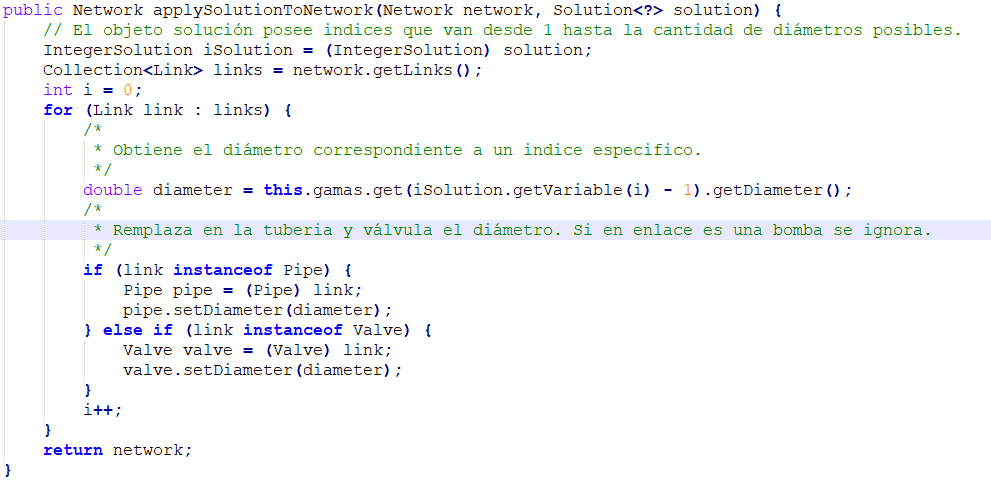
\includegraphics[width=\textwidth]{Seccion2/assets/applySolutionToNetwork.png}
    \caption{Ejemplo del m�todo \textit{applySolutionToNetwork}.}
    \label{fig:applySolutionToNetwork}
\end{figure}
